\newpage
\section{Model-To-Tree with TGGs}
\genHeader

One powerful benefit of working with TGG transformations is that by specifiying one transformation (i.e., a forward transformation), we're able to get the
opposite direction for free! Our example used a \texttt{tree.xmi} (\texttt{MocaTree}
instance) input, transformed it forward into \texttt{tree.xmi\_fwd.xmi} (\texttt{Dictionary} instance), and used that result file in a backwards
transformation to create the final tree output, \texttt{tree.xmi\_FWD.xmi\_BWD.xmi}, all without error! If our TGG was truly successful however,
the starting and final files should be identical. Let's compare the two (Fig.~\ref{eclipse:comparingTreeModels}).

\vspace{0.5cm}

\begin{figure}[htpb]
\begin{center}
  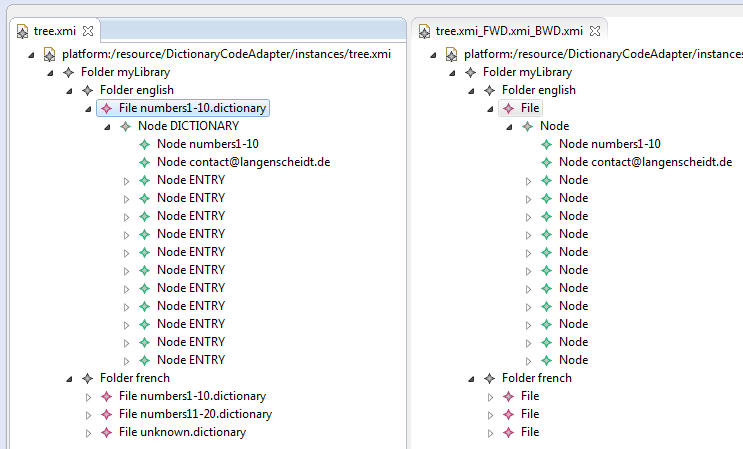
\includegraphics[width=\textwidth]{eclipse_generatedBackwardsModel}
  \caption{Not yet identical trees}
  \label{eclipse:comparingTreeModels}
\end{center}
\end{figure}

\vspace{0.5cm}

It's close, but not perfect. You can see that some things need to be refined. The ``DICTIONARY'' and ``ENTRY'' labels, for example, are missing from the
major nodes. We need to include an attribute constraint to bind these specific EString values. You'll also notice that, as you scroll through each
\texttt{Node}, the \texttt{title} and \texttt{author} nodes have the correct \texttt{index} values of 0 and 1, but the remaining \texttt{entry} indices are also
set to 0.
We were only concerned with binding the title and author nodes in the forward direction, as we could assume that any other node with any other index value (2 and greater) was an
\texttt{entryNode}. In the backwards direction however, this distinction is lost, which means we must introduce a custom attribute constraint.

\jumpDual{m2tvis}{m2ttex}

\newpage
\hypertarget{m2tvis}{}
\subsection{Double-checking the TGG}
\visHeader

\begin{itemize}

\item[$\blacktriangleright$] Open \texttt{NodeToDictionaryRule} and update as depicted below (via attribute constraint). Is this in the right place? Should this
be done before??

\begin{figure}[htp]
\begin{center}
  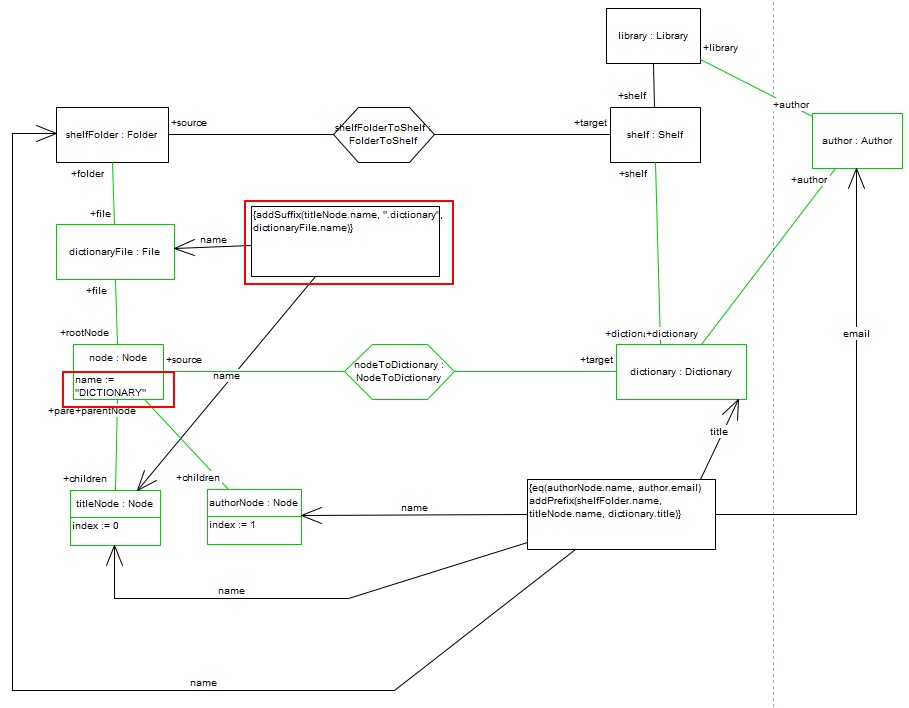
\includegraphics[width=\textwidth]{ea_updateNodeToDictionary}
  \caption{updated NodeToDictionary}
  \label{ea:NodeToDictionary_updated}
\end{center}
\end{figure}

\item[$\blacktriangleright$] Similarly, open \texttt{ForAllEntry} in EA and update like so:

\begin{figure}[htp]
\begin{center}
  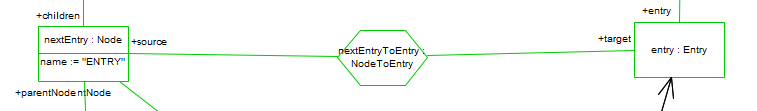
\includegraphics[width=\textwidth]{ea_updateForAllEntry}
  \caption{updated ForAllEntry}
  \label{ea:ForAllEntry_updated}
\end{center}
\end{figure}

\item[$\blacktriangleright$] End comment.

\jumpSingle{finalStep}

\end{itemize}


\newpage
\hypertarget{m2ttex}{}
\subsection{Refining the TGG Transformation}
\texHeader

\begin{itemize}

\item[$\blacktriangleright$] Find the relevant files and add the following attribute constraints. Note : the MOSL parser requires that all attribute constraints
are declared before link variables.

\begin{figure}[htp]
\begin{center}
  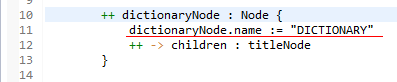
\includegraphics[width=0.8\textwidth]{eclipse_NodeToDictionaryRule_updated}
  \caption[labelInTOC]{needs refinement\ldots}
  \label{eclipse:generatedBkwrdMdl}
\end{center}
\end{figure}

\begin{figure}[htp]
\begin{center}
  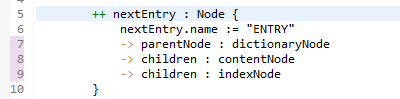
\includegraphics[width=0.8\textwidth]{eclipse_ForAllEntryRule_updated}
  \caption[labelInTOC]{needs refinement\ldots}
  \label{eclipse:generatedBkwrdMdl}
\end{center}
\end{figure} 

\item[$\blacktriangleright$] Add new SetDefaultNumber CSP here.

\begin{figure}[htbp]
\begin{center}
  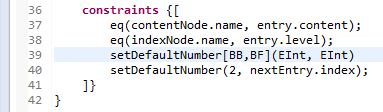
\includegraphics[width=0.6\textwidth]{eclipse_setDefaultNumberConstraint}
  \caption{extra constraint}
  \label{eclipse:newEntryConstraint}
\end{center}
\end{figure}

\end{itemize}


\newpage
\hypertarget{common cspConstraint}{}
\subsection{Implementing SetDefaultNumber}
\genHeader

We've declared and used our custom \texttt{SetDefaultNumber} constraint, but we haven't given it any implementation code yet. If you haven't yet, save and build
\texttt{DictionaryCodeAdapter} before continuing.

\begin{itemize}

\item[$\blacktriangleright$] Navigate to ``/src,'' where a new \texttt{csp.constraints} package was generated, and open \texttt{SetDefaultNumber.java}. Edit
this file until it matches Fig.~\ref{eclipse:setDefaultImpl}.

\begin{figure}[htbp]
\begin{center}
  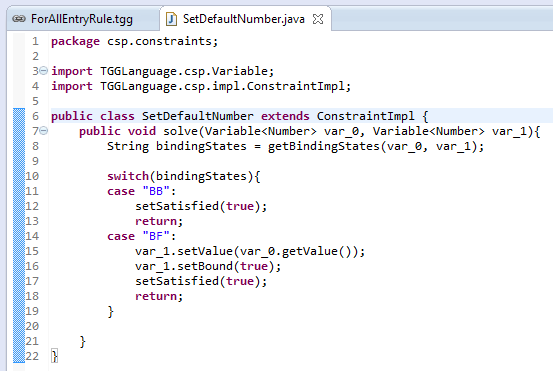
\includegraphics[width=0.9\textwidth]{eclipse_setDefaultNumberImplementation}
  \caption{extra constraint impl}
  \label{eclipse:setDefaultImpl}
\end{center}
\end{figure}

\item[$\blacktriangleright$] Save, build, and run \texttt{TGGMain} one more time. The inital and final \texttt{tree} variants should now be nearly identical! If
you're worried about some of the nodes being in the wrong order (such as an author at the bottom of the list), double-click on them and check their
\texttt{index} properties. If everything has been done correctly every \texttt{entry} should be 2, each \texttt{author} should be 1, and each \texttt{title}
should be 0.

\item[$\blacktriangleright$] On a final note to end the model-to-text step, wasn't it great how easy and short this was? If we were to use another
transformation set up (such as SDMs), we would have had to create independent rules for this backwards direction. Instead, TGGs gave us this transform for free!

\end{itemize}

